%----------------------------------------------------------------------------------------
%	CHAPTER 3
%----------------------------------------------------------------------------------------
\chapterimage{ChapterImages/chapter3.png} % Chapter heading image

\chapter{File Permissions and Access Control}
\label{ch:permissions}

In Linux, every file and directory carries a set of permissions that decide who can read it, change it, or run it. This chapter builds on the users and groups introduced in Chapter~\ref{ch:users-groups}: permissions are what actually put those user and group identities to work, controlling access at the level of individual files and directories.

\section{Understanding Permissions}

In Linux, every file and directory has three types of permissions:
\begin{enumerate}
    \item \textbf{Read (\texttt{r})} -- permission to view the contents of a file, or list the contents of a directory.
    \item \textbf{Write (\texttt{w})} -- permission to modify a file, or create/delete entries inside a directory.
    \item \textbf{Execute (\texttt{x})} -- permission to run a file as a program, or enter (\texttt{cd} into) a directory.
\end{enumerate}

These permissions are tracked separately for the file's \textbf{owner}, its \textbf{group}, and \textbf{other} users, and are displayed together as a 10-character string such as \texttt{-rwxr-xr--}. Figure~\ref{fig:permission-bits} breaks this string down.

\begin{figure}[h]
    \centering
    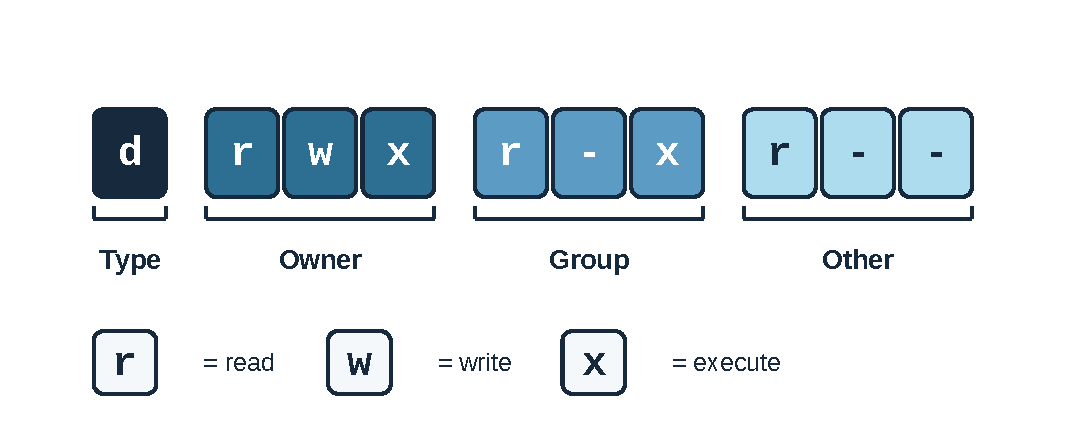
\includegraphics[width=0.85\textwidth]{Images/Chapter3/permission-bits.pdf}
    \caption{Anatomy of a permission string: file type, followed by owner, group, and other permissions.}
    \label{fig:permission-bits}
\end{figure}

\textbf{Example:} \texttt{-rwxrw-r--}
\begin{itemize}
    \item Owner: can read, write, and execute the file.
    \item Group: can read and write the file, but not execute it.
    \item Other users: can only read the file.
\end{itemize}
The leading character shows the entry type: \texttt{-} for a regular file, \texttt{d} for a directory (other values exist for links and devices, which are outside the scope of this lab).

\textbf{Displaying Permissions:}
\begin{lstlisting}[language=Terminal]
$ ls -l file.txt
\end{lstlisting}

\section{Changing Permissions}

\begin{enumerate}
    \item \textbf{Symbolic mode:}\\
    \texttt{+} adds a permission, \texttt{-} removes a permission, \texttt{=} sets the permission exactly (removing any others).
\begin{lstlisting}[language=Terminal]
$ chmod u+x file.sh    # owner gets execute permission
$ chmod g-w file.txt   # remove write permission from the group
$ chmod o=r file.txt   # others get read-only, nothing else
\end{lstlisting}

    \item \textbf{Octal (numeric) mode:} each permission has a numeric value -- \texttt{r = 4}, \texttt{w = 2}, \texttt{x = 1} -- and the three are added together for each of owner/group/other.
\begin{lstlisting}[language=Terminal]
$ chmod 754 script.sh
\end{lstlisting}
    This means:\\
    Owner: $7 = 4+2+1 \rightarrow$ \texttt{rwx}\\
    Group: $5 = 4+0+1 \rightarrow$ \texttt{r-x}\\
    Other: $4 = 4+0+0 \rightarrow$ \texttt{r--}

    \item \textbf{Changing ownership:}
\begin{lstlisting}[language=Terminal]
$ sudo chown username file.txt              # change the file's owner
$ sudo chown username:groupname file.txt    # change owner and group together
$ sudo chgrp groupname file.txt             # change only the group
\end{lstlisting}
\end{enumerate}

\section{Special Permissions}
Beyond the standard \texttt{rwx} bits, Linux defines \textbf{three special permissions} for specific capabilities:

\begin{enumerate}
    \item \textbf{SUID (Set User ID):} when an executable file with the SUID bit set is run, it executes with the privileges of the file's \emph{owner}, not the user who launched it.\\
    Symbolic: \texttt{-rwsr-xr-x} -- the \texttt{s} replaces the owner's \texttt{x}.\\
    Numeric: \texttt{chmod 4755 /path/to/exe} -- the leading \texttt{4} sets SUID.

    \item \textbf{SGID (Set Group ID):}
    \begin{itemize}
        \item On a file: it executes with the privileges of the file's \emph{group}.
        \item On a directory: new files created inside automatically inherit that directory's group, which is very useful for shared team folders.
    \end{itemize}
    Symbolic: \texttt{drwxrws---} -- the \texttt{s} replaces the group's \texttt{x}.\\
    Numeric: \texttt{chmod 2750 /opt/project} -- the leading \texttt{2} sets SGID.

    \item \textbf{Sticky Bit:} typically used on shared directories (e.g.\ \texttt{/tmp}); it restricts deletion so that only a file's owner (or root) can remove it, even if others have write access to the directory.\\
    Symbolic: \texttt{drwxrwxrwt} -- the \texttt{t} replaces the others' \texttt{x}.\\
    Numeric: \texttt{chmod 1777 /tmp} -- the leading \texttt{1} sets the Sticky Bit.
\end{enumerate}

\textbf{Note:} These leading digits can be combined, e.g.\ \texttt{chmod 6755} sets both SUID and SGID.

\section{Access Control Lists (ACL)}
Standard Unix permissions only distinguish owner/group/other, which is not always flexible enough. \textbf{ACLs} let you assign different permissions to any number of individual users or groups on the same file.

\begin{enumerate}
    \item \textbf{Viewing an ACL:}
\begin{lstlisting}[language=Terminal]
$ getfacl file.txt
\end{lstlisting}

    \item \textbf{Adding ACL permissions:}
\begin{lstlisting}[language=Terminal]
$ setfacl -m u:alice:rwx file1.txt   # grant alice rwx on file1.txt
$ setfacl -m g:staff:r-- file1.txt   # grant group "staff" read-only
\end{lstlisting}

    \item \textbf{Setting a default ACL for a directory} (applied automatically to new files created inside it):
\begin{lstlisting}[language=Terminal]
$ setfacl -dm u:username:rwx dir/
\end{lstlisting}

    \item \textbf{Removing ACL entries:}
\begin{itemize}
    \item Remove one user's entry: \texttt{setfacl -x u:alice file.txt}
    \item Remove one group's entry: \texttt{setfacl -x g:staff file.txt}
    \item Remove all ACL entries (revert to standard permissions): \texttt{setfacl -b file.txt}
\end{itemize}
\end{enumerate}

\section*{Important Notes}
Any command that modifies system files or user/group settings usually \textbf{requires} \texttt{sudo} -- this includes \texttt{groupadd}, \texttt{useradd}, \texttt{setfacl}, \texttt{chown}, and \texttt{chmod} on files you do not own. Read-only commands such as \texttt{getfacl}, \texttt{ls}, \texttt{groups}, and \texttt{id} do \textbf{not} require \texttt{sudo}, unless the target file's permissions already block your user from reading it.
